\section{OneMax}
\subsection{Code Description}
	Out EA code is based around a set of \textit{interfaces} and \textit{abstract classes} as seen in figure~\ref{fig:classes}.
	The configuration is managed by \textit{OneMax} and \textit{ColonelBlotto} themselfs, before invoking the EA loop.
	\begin{figure}[H]
		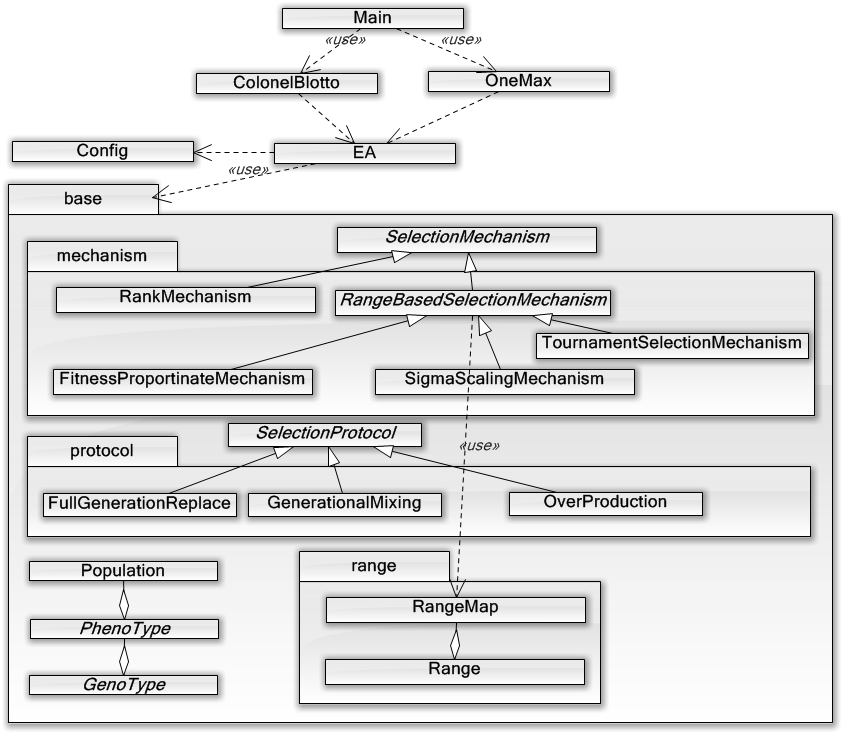
\includegraphics[width=\columnwidth]{images/ClassStructure.png}
		\caption{Class structure}
		\label{fig:classes}
	\end{figure}
	The EA loop consists of four main stages: development, adult selection, parent selection and reproduction. In this exercise only a selection protocol is used for adult selection, and a selection mechanism used for parent selection. Development is handled by the specific genotype depending on the task at hand, and reproduction is handled by the EA class which includes the crossover and mutation rates. 
	
\subsection{Code Modularity and reusabulity}
	Every main component of our EA project is based on an interface or abstract class (with the exception of EA itself). In order to implement your own version you just have to implement the missing functionality described in these base classes.\\\\
SelectionMechanism example:
	\begin{verbatim}
public class ExampleMechanism extends SelectionMechanism {
    @Override
    protected PhenoType getMate() {
        //Your logic here
    }
}
	\end{verbatim}
	SelectionProtocol example:
	\begin{verbatim}
public class ExampleProtocol implements SelectionProtocol {
    public Population<PhenoType> selection(Population<PhenoType> adults, Population<PhenoType> children, int max) {
        //Your logic here
    }
    public int childrenNeeded(int populationSize) {
        //Your logic here
    }
}
	\end{verbatim}
	Similar procedures can be used for \textit{GenoType} and \textit{PhenoType}.
\subsection{Code Performance on 40-bit One-Max}
	In order to consistenly find a solution in under 100 generations required a population size of 400. When experimenting with the crossover and mutation rates we discovered that they yielded best result when set to 0.9 and 0.01 respectively. This can be seen in the graphs below:
	\begin{figure}[H]
	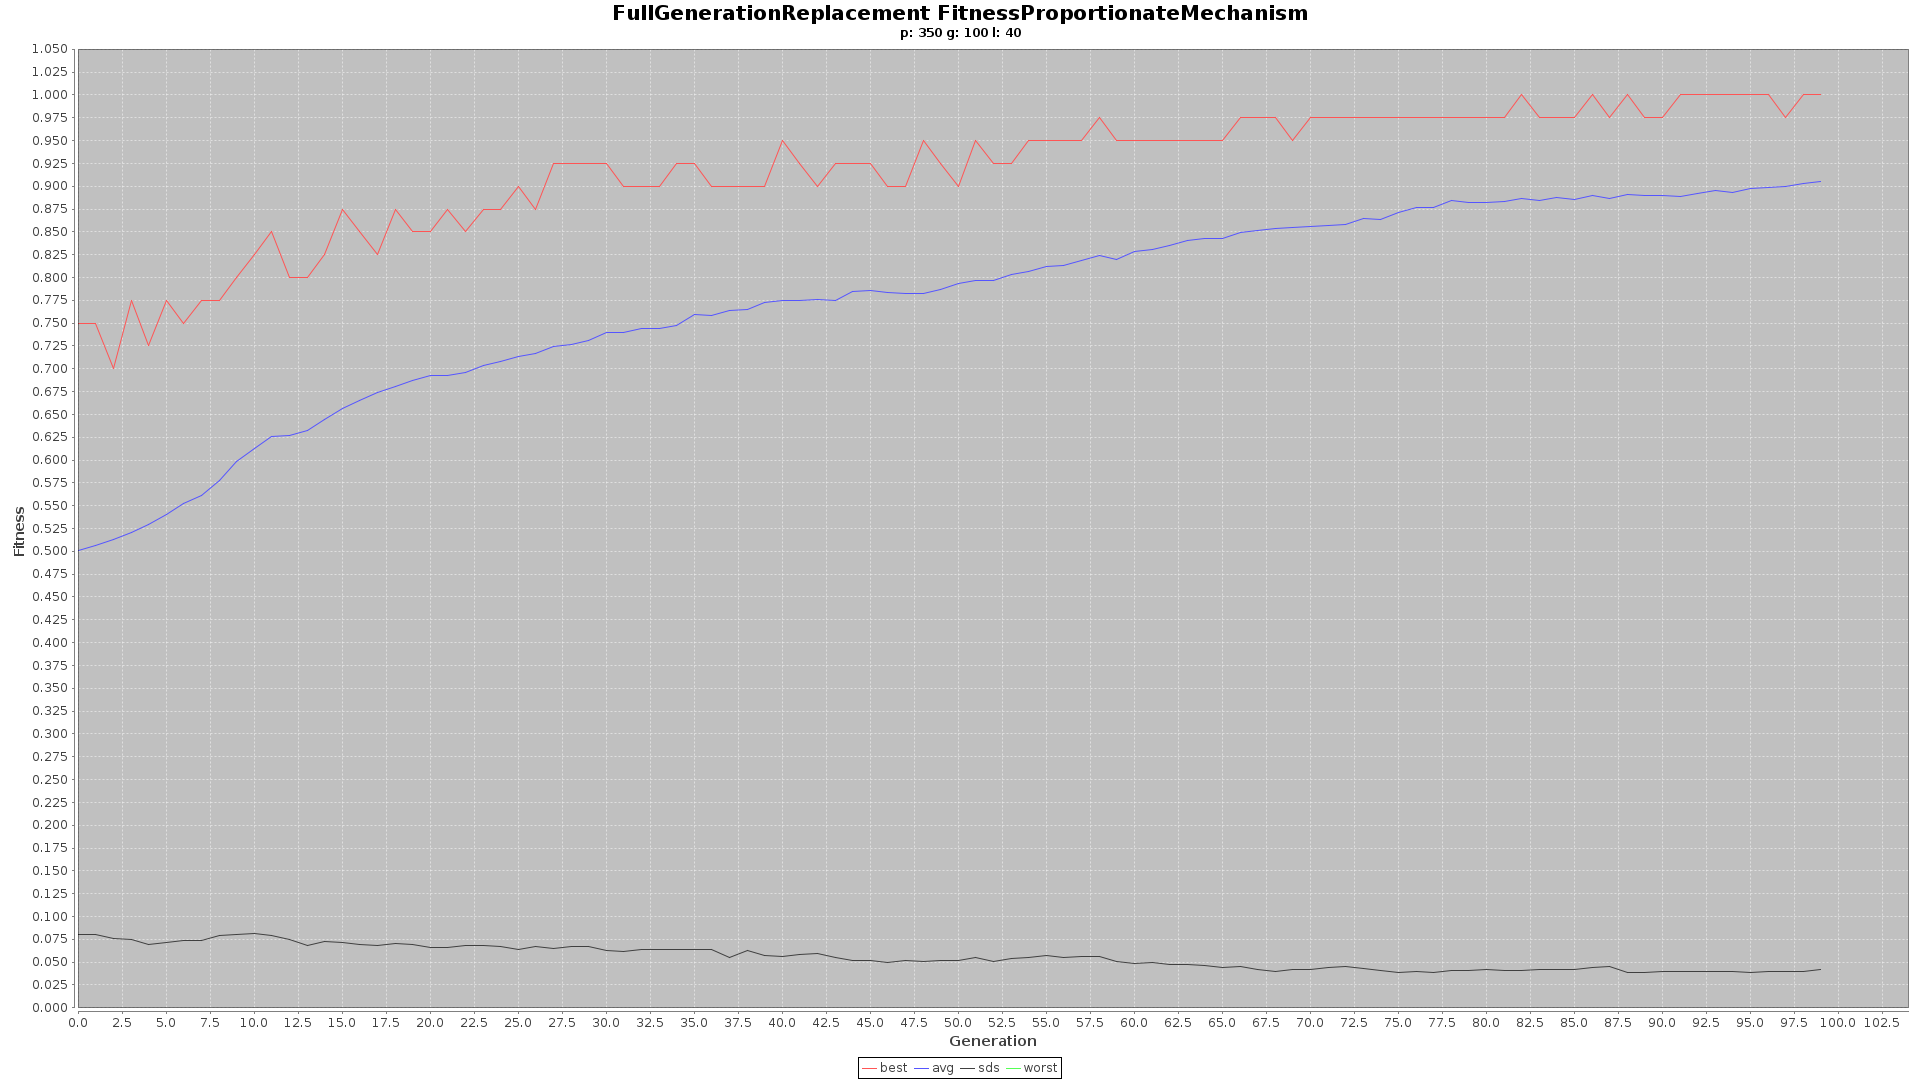
\includegraphics[width=\columnwidth]{1/c/350.png}%
	\caption{population 350, cr 0.9, m 0.01}%
	\label{fig:350}%
	\end{figure}
	\begin{figure}[H]%
	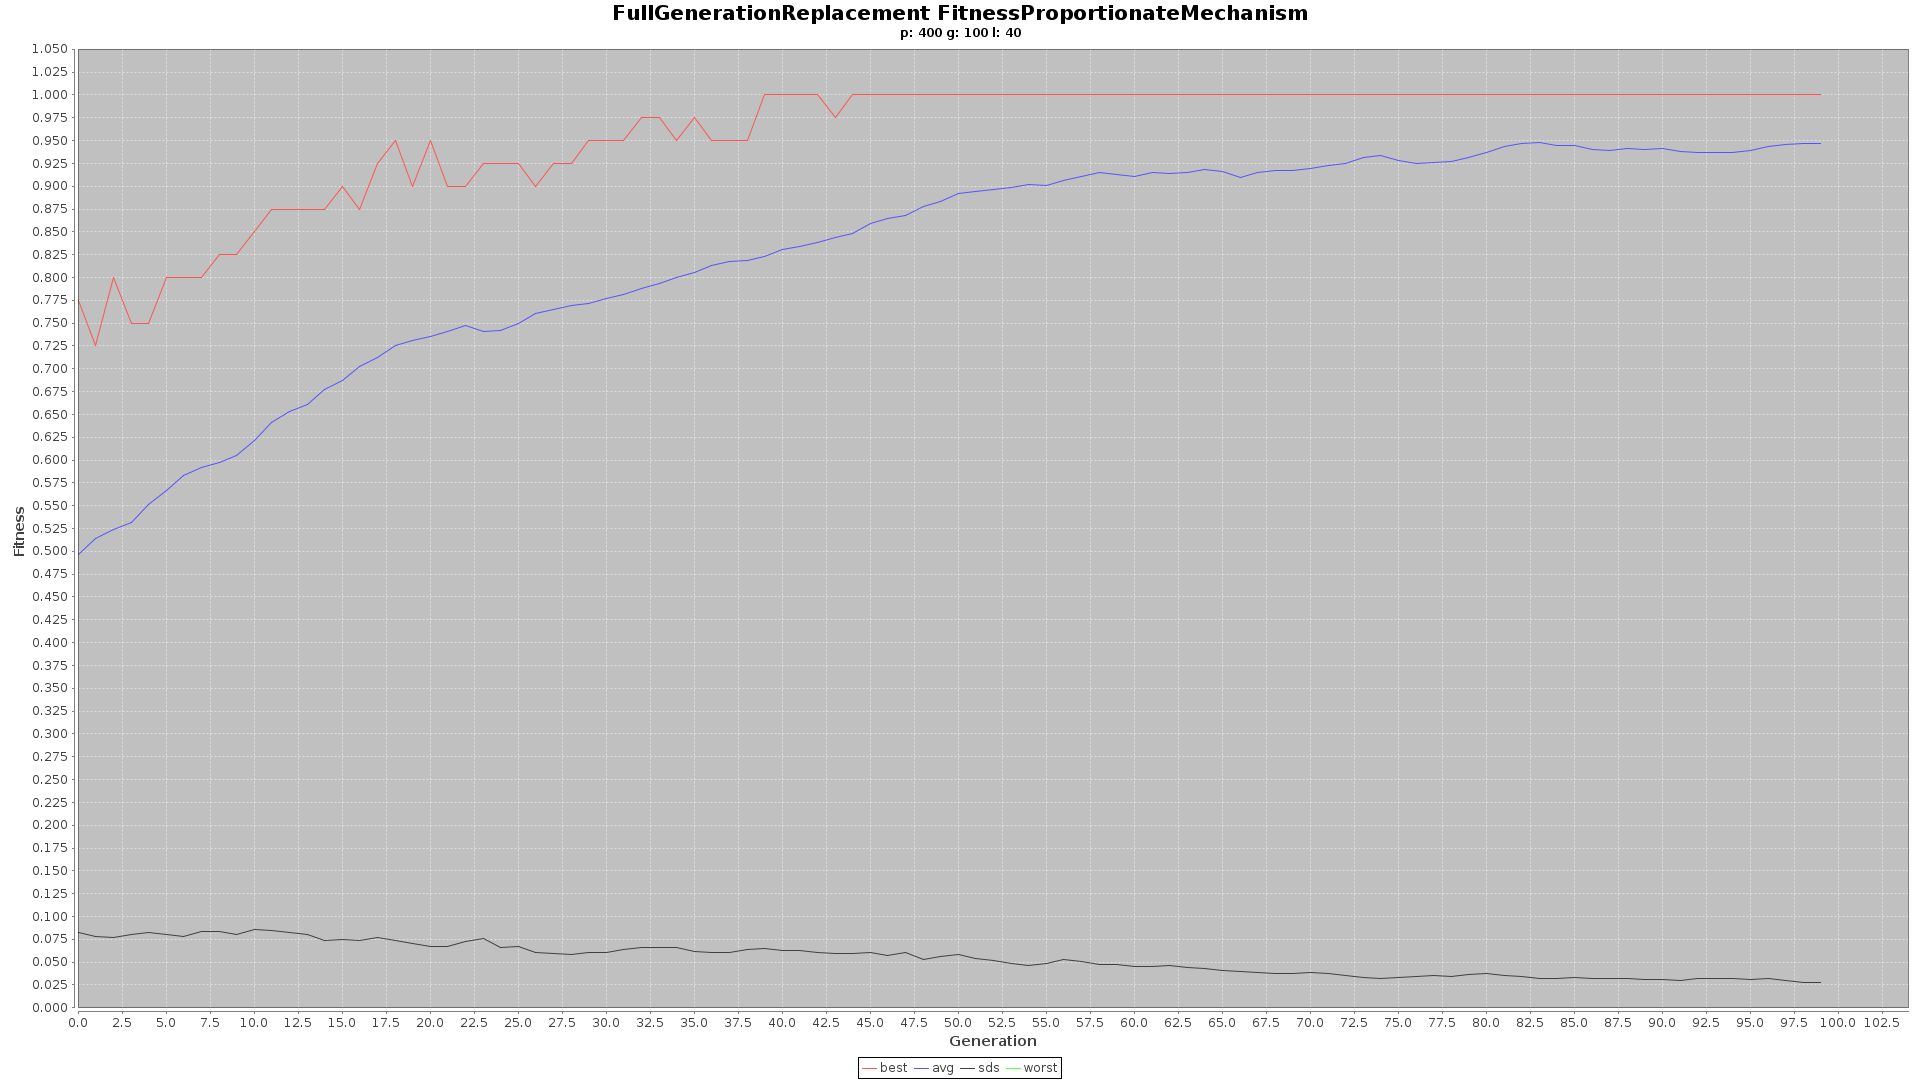
\includegraphics[width=\columnwidth]{1/c/400.png}%
	\caption{population 400, cr 0.9, m 0.01}%
	\label{fig:400}%
	\end{figure}
	
\subsection{Parent selection}
	When trying all possible permutations of selection protocols and mechanism while using the best found settings from the previous experiment we found that the combination of generational mixing or overproduction with a tournament selection mechanism yielded the best result. See figure~\ref{fig:gen} and~\ref{fig:over}
	\begin{figure}[H]%
	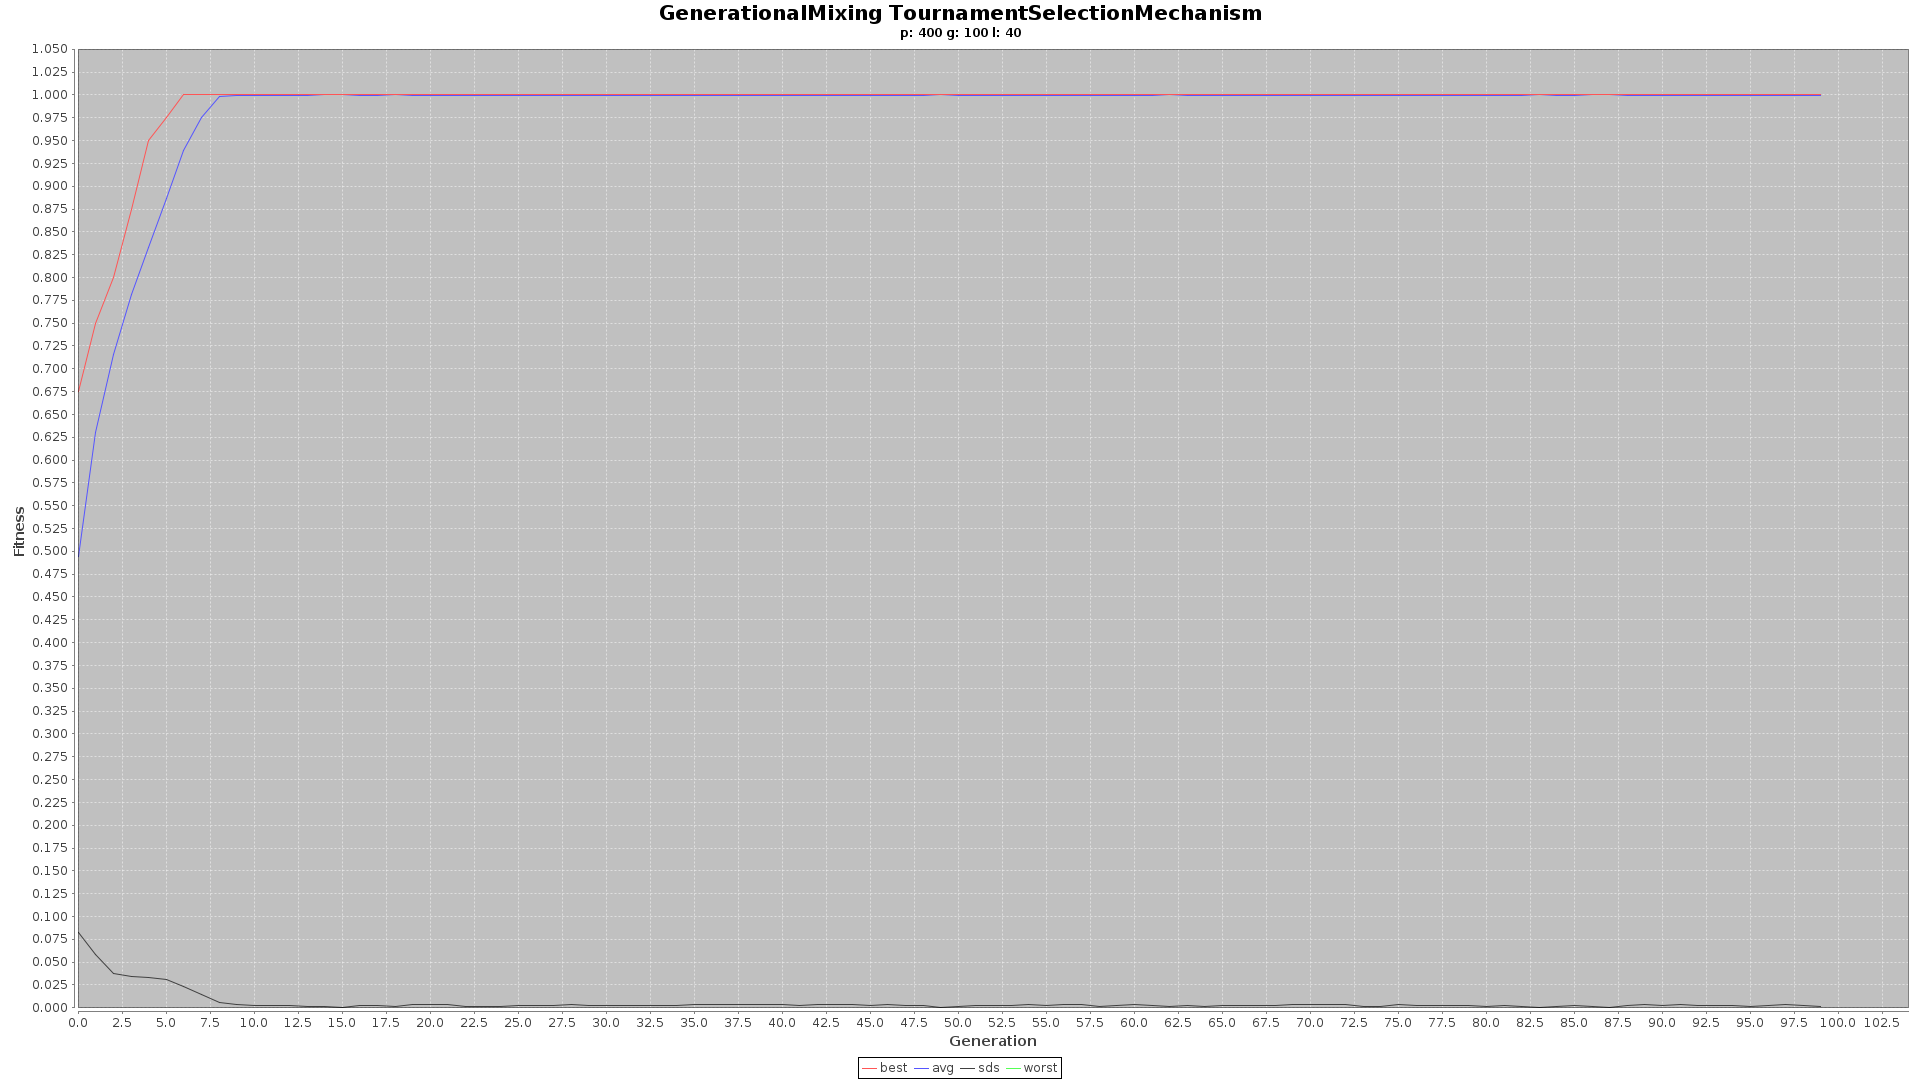
\includegraphics[width=\columnwidth]{1/d/gen.png}%
	\caption{Generational mixing with tournament selection}%
	\label{fig:gen}%
	\end{figure}
	\begin{figure}[H]%
	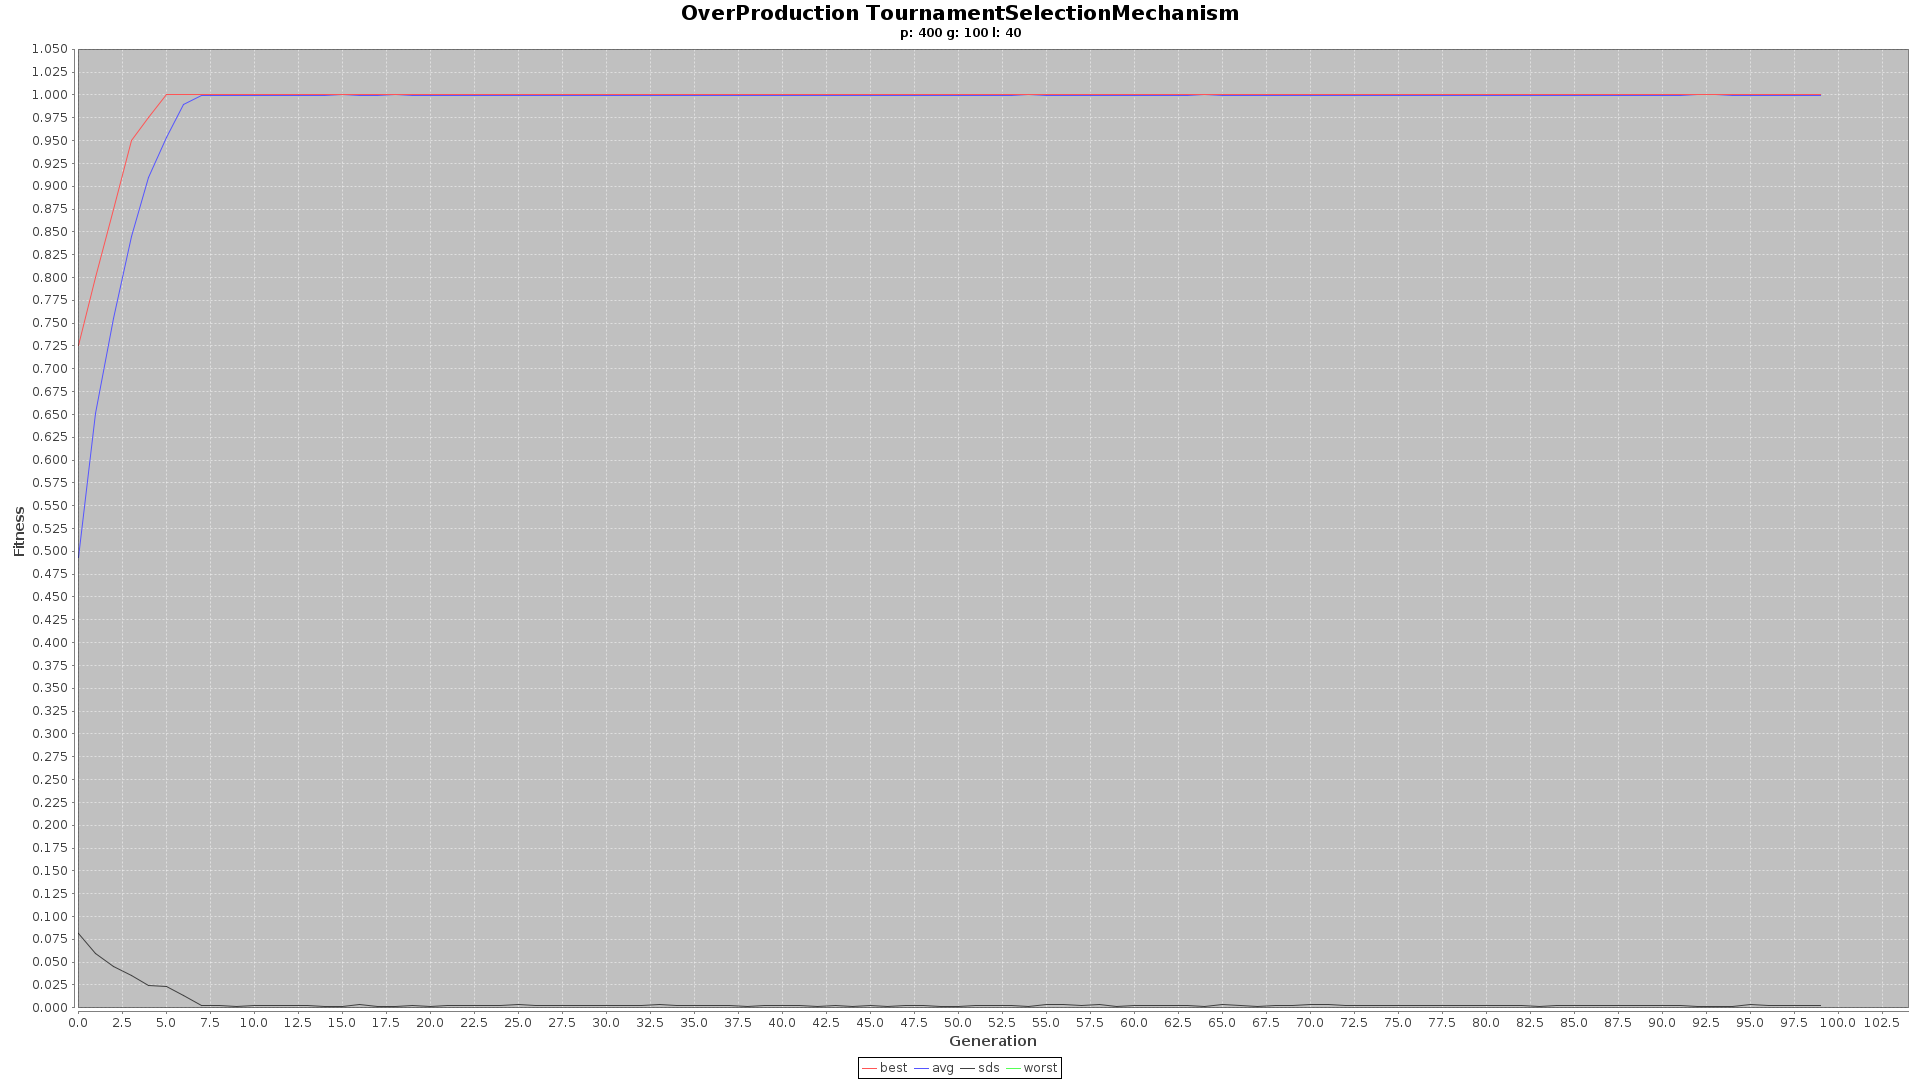
\includegraphics[width=\columnwidth]{1/d/over.png}%
	\caption{Overproduction with tournament selection}%
	\label{fig:over}%
	\end{figure}
\subsection{Random goal}
	Using the same settings as the previous experiment, except using a random bitvector of length 40, we experienced the same results in general. Which is to be expected because evolution differentiate between different solutions, and will always strive to increase the fitness of a population regardless of the final solution(based on a generalized fitness rule). We ran multiple different runs to verify our observation, one which can be viewed in figure~\ref{fig:random}
	\begin{figure}[H]%
	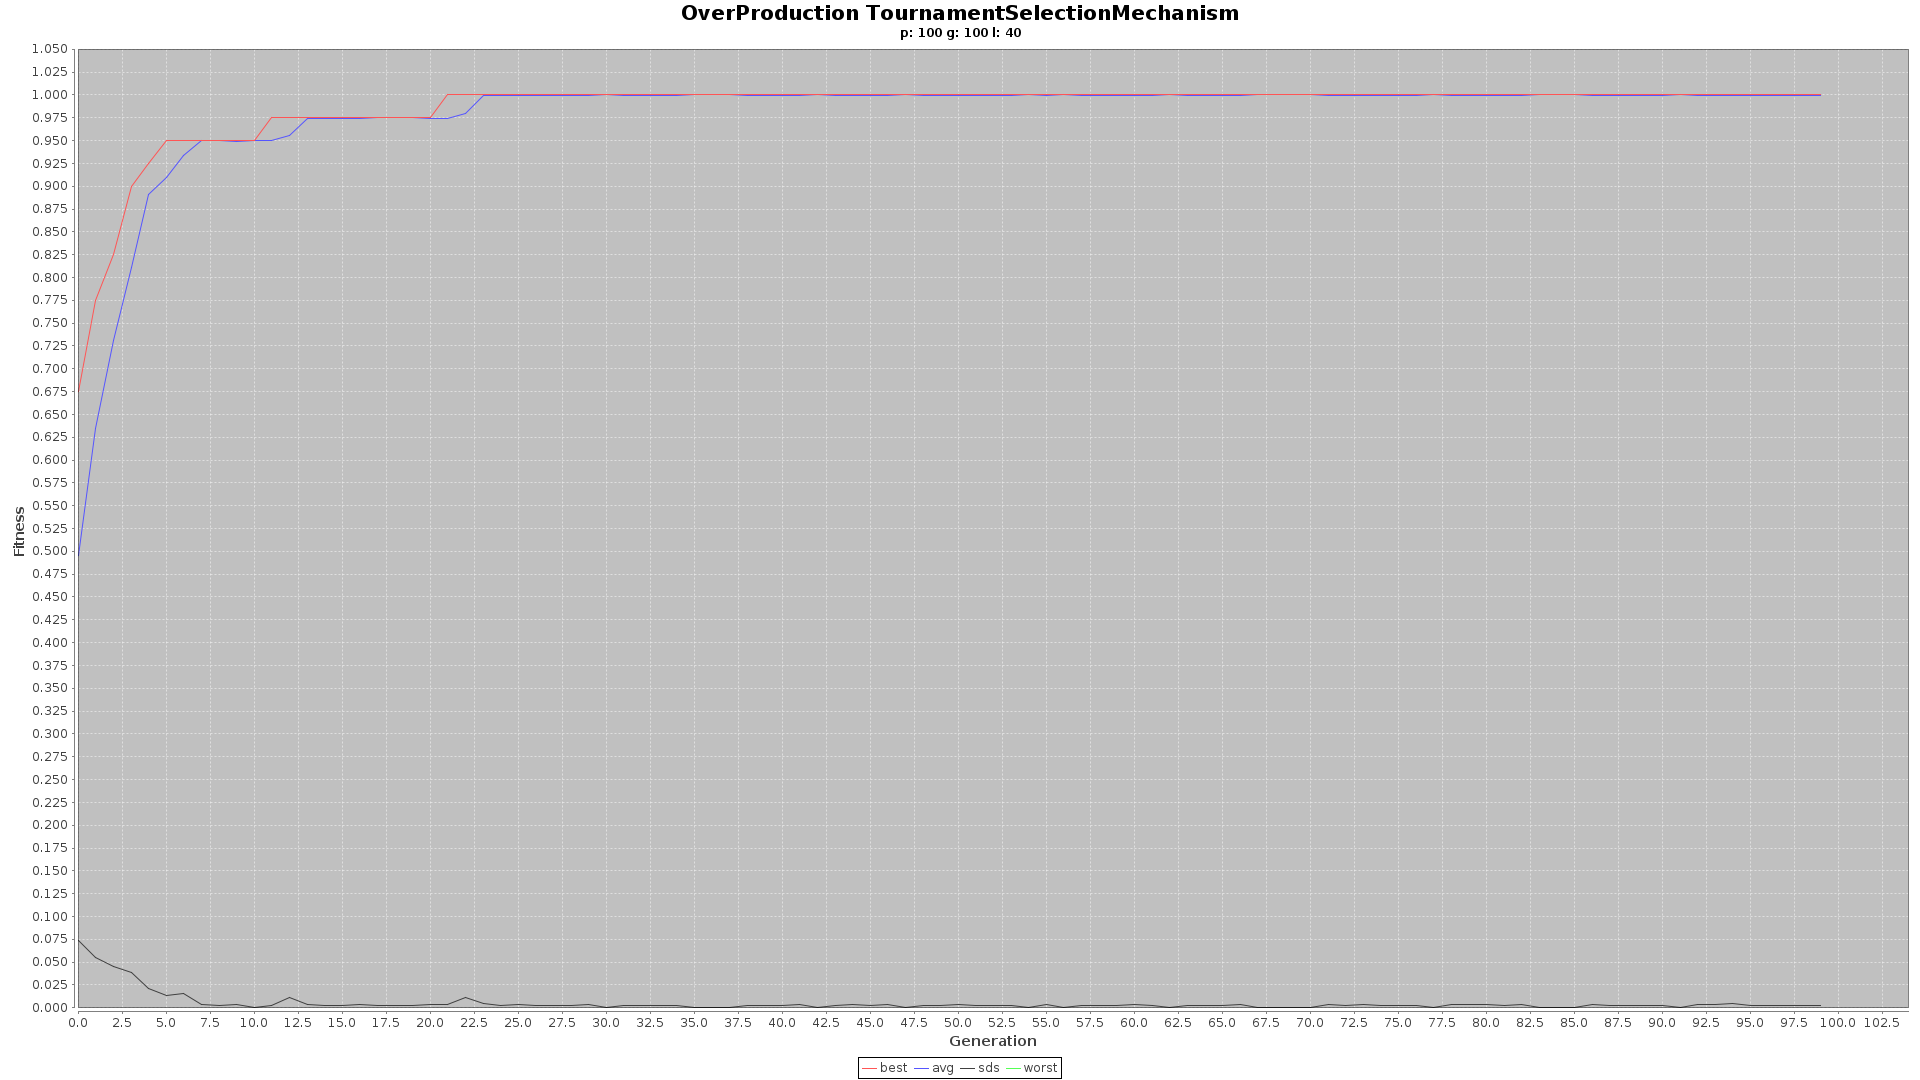
\includegraphics[width=\columnwidth]{1/e/random.png}%
	\caption{Overproduction with tournament selection towards a random goal}%
	\label{fig:random}%
	\end{figure}
	When running this several consecutive times we achived similar results, each resulting in a stable solution at around generation 25. 